\chapter{Experimentální uspořádání}

\section{Optické měřící přístroje}

\subsection{Bruker VERTEX 80v}
Jedná se o je vakuový FTIR spektrofotometr, který obsahuje Michelsonův interferometr, se zrcadlem kmitajícím na vzduchovém polštáři. Během všech měření byl používán speciální nástavec, díky němuž bylo možné provádět správné absolutní měření propustnosti. V průběhu měření jsou vzorky umístěny svisle na držáku v měřící komoře, ve které je po dobu měření udržováno vakuum 2,51\,hPa, což slouží k minimalizace vlivu okolního prostředí a vlhkosti na průběh měření. Výrobcem udávaní spektrání rozlišení spektrometru je minimálně 0,2\,cm$^{-1}$ při běžných laboratorních podmínkách. Spektrální rozsah spektrofotometru je 1333 -- 27000\,cm$^{-1}$, ale při požití vhodných rozšíření je možné měřit i do FIR a UV/VIS oblastí \cite{vertex}.

FIXME: Vyfotit obrázek.

%\begin{figure}
%  \centering
%  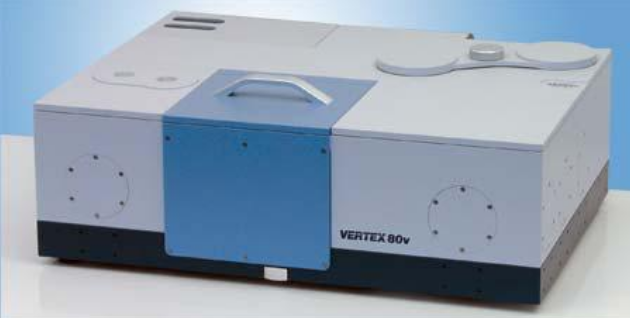
\includegraphics[width=120mm]{vertex80v.png}
%  \caption{Spektrofotometr Bruker VERTEX 80v.}
%  \label{verteximg}
%\end{figure}

\subsection{LAMBDA 1050 UV/Vis/NIR}
LAMBDA 1050 UV/Vis/NIR od firmy PerkinElmer je dvoukanálový spektrofotometr. Jako zdroj slouží halogen-rtuťová a deuteriová lampa.  Přístroj obsahuje dva monochromátory (holografické difrakční mřížky s 1440 proužky,vrypy? na milimetr pro UV/Vis oblast a s 360 proužky na milimetr pro IR oblast)  (FIXME: holographic grating monochromator with 1440 lines/mm UV/Vis blazed at 240 nm and 360 lines/mm NIR blazed at 1100 nm,). Pro dělení svazku na dva kanály je použit chopper. Udávaný spektrální rozsah je 175--3300\,nm, nicméně pro měření pod 185\,nm je potřeba chlazení dusíkem. Použitý detektor pro viditelnou a UV oblast je fotonásobič R6872. Pro oblast 860--1800\,nm je použit InGaAs detektor, chlazený peltierovým článkem a pro oblast 1800--2500\,nm PbS detektor, taktéž chlazený peltierovým článkem. Spektrální rozlišení výrobce udává jako minimálně 0,05\,nm. Přístroj obsahuje optickou kompenzaci pro různé tloušťky vzorků \cite{lambda}.

FIXME: Vyfotit obrázek.

%\begin{figure}
%  \centering
%  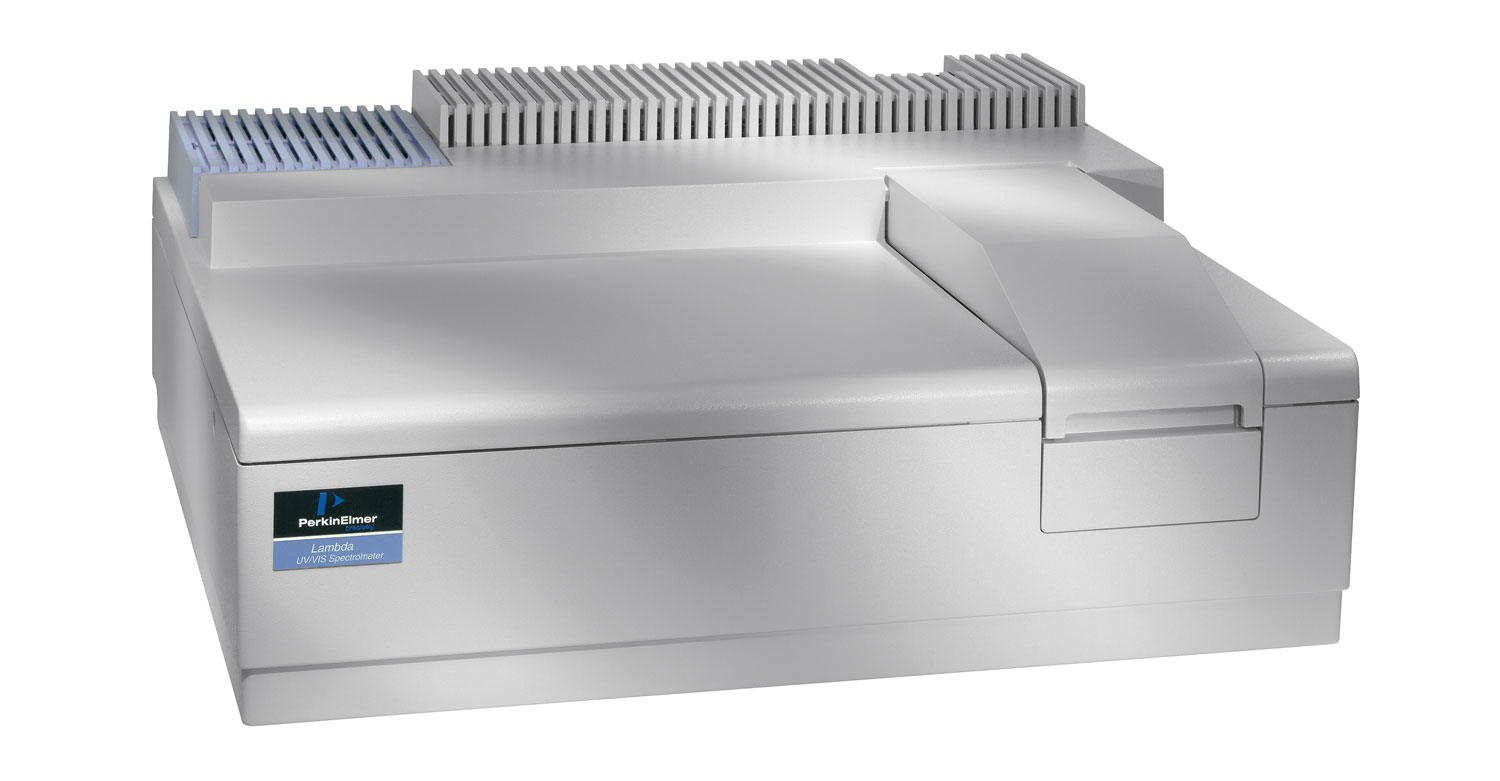
\includegraphics[width=120mm]{LAMBDA.jpg}
%  \caption{Spektrofotometr LAMBDA 45 UV/Vis.}
%  \label{lambdaimg}
%\end{figure}

\subsection{Jobin-Yvon UVISEL}
Schéma elipsometru Jobin-Yvon UVISEL je znázorněno na schématu (FIXME: udělat schéma v inkscapu). Udávaný spektrální rozsah tohoto přístroje je od 190\,nm do 2000\,nm. Hlavy elipsometru jsou umístěny na goniometru, z toho důvodu může být měření prováděno pod různými úhly. Běžně se měří úhly dopadu 55$^\circ$, 60$^\circ$, 65$^\circ$, 70$^\circ$ a 75$^\circ$. Jedná se o fázově modulovaný elipsometr. Měření probíhá tak, že z lampy vychází nepolarizované polychromatické světlo, které poté prochází přes polarizátor. Tam dojde k jeho lineární polarizaci, odráží se od vzorku a přes kompenzátor, analyzátor a monochromátor dopadá na detektor.

FIXME: Taky možná fotku?

%\begin{figure}
%  \centering
%  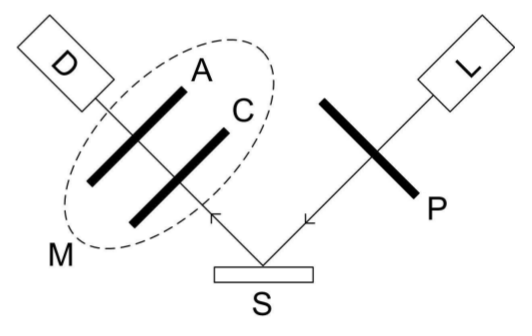
\includegraphics[width=120mm]{schema-elipsometru.png}
%  \caption{Schéma elipsometru UVISEL (P--polarizátor, C--kompenzátor, D--detektor, L--lampa, M--modulátor, A--analyzátor, S--substrát), obrázek převzat z \cite{fialova2009}.}
%  \label{fig:elipsometrimg}
%\end{figure}

\section{Depoziční aparatura}
FIXME:tohle je v podstatě opsáno z bakalářky... zkontrolovat jestli to všechni stále sedí!

Všechny vrstvy byly deponovány na Ústavu fyzikální elektroniky Masarykovy University v reaktoru R2. 

Reaktor R2 je válcový ocelový reaktor a má planární elektrody. Jeho vnitřní průměr je 49\,cm a má výšku 24,6\,cm. Horní i dolní elektroda jsou kruhového tvaru. Průměr horní elektrody je 38\,cm, průměr dolní elektrody pak 40\,cm. Horní elektroda je uzemněná. Plyny používané při depozici jsou do reaktoru přiváděny přes otvory v horní elektrodě, kde jsou rozmístěny středově symetricky v kru\-hu o průměru 18\,cm. Deponovaný vzorek je umístěn přímo na dolní elektrodě. Na dolní elektrodu je také přiváděno vysokofrekvenční napětí. Jako zdroj RF napětí byl použit generátor Cesar 133 firmy Dressler pracující na frekvrenci 13,56\,MHz.

Tlak v aparatuře je měřen kapacitronem Leybold. Průtoky plynů do reaktoru jsou regulovány průtokoměry Hastlings. 

\section{Depoziční podmínky}

Nezávislé depožiční podmínky pro všechny depozice jsou tlak $p$, výkon $P$, čas depozice $t$ a průtoky jednotlivých plynů $Q_{\mathrm{CH_4}}$, $Q_{\mathrm{H_2}}$, $Q_{\mathrm{Ar}}$, všechny depoziční podmínky jsou shrnuty v tabulce \ref{deppodminky}. Předpětí $U_b$ pak není nezávislý parametr, ale závisí na výkonu přibližně jako $U_b \sim \sqrt{P}$, nicméně je také zahrnuto v tabulce protože se jedná o velmi důležitý parametr pro růst vrstvy. Klíčový parametr, jak již bylo zmíněno v Kapitole jedna je především energie dopadajícího iontu v přepočtu na jeden atom. Předpětí $U_b$ tedy říká, jakou energii by měl ion po průletu stěnovou vrstvou, kdyby nedocházelo ke srážce. Bohužel ve skutečnosti se ukazuje, že závislost $U_b$ na ostatních depozičních podmínkách není moc dobře reprodukovatelná, což je z tabulky \ref{deppodminky} jasně patrné. Nejstarší vrstvy jsou totiž z roku 2008 a nejnovější z konce roku 2012, v průběhu let potom mohlo dojít na aparatuře například ke stárnutí zdroje a také třeba ke změnám v reaktrou (deponování vrstvy na stěnách a elektrodách atd.). 

\begin{table}[htbp]
 \centering
 \begin{tabular}{lccccccc}
	\hline
	{Vrstva} & {$p$\,[Pa]} & {$P$\,[W]} & {$U_b$\,[V]} & {$t$\,[min]} & {$Q_{\mathrm{CH_4}}$} & {$Q_\mathrm{H_2}$} & {$Q_\mathrm{Ar}$} \\
	& & & & & {[sccm]} & {[sccm]} & {[sccm]} \\
	\hline\hline
	CH30A     & 12 & 100 & 75  & 30   & 8,7 & 5 & 0 \\
	CH30A\_280 & 12 & 100 & 75  & 30   & 8,7 & 5 & 0 \\
	CH30A\_340 & 12 & 100 & 75  & 30   & 8,7 & 5 & 0 \\
	CH83A     & 12 & 75  & 115 & 120  & 8   & 0 & 5 \\
	CH87A     & 8  & 60  & 120 & 120  & 8   & 5 & 0 \\
	CH88A     & 8  & 60  & 140 & 4*30 & 8   & 5 & 0	\\
	CH90A     & 8  & 65  & 145 & 30   & 8   & 5 & 0 \\
	\hline
 \end{tabular}
 \caption{Depoziční podmínky, Q$_\mathrm{{HMDSO}}$ je průtok HMDSO, Q$_\mathrm{O2}$ je průtok kyslíku, $P$ je výkon, $U_b$ je samopředpětí, $p$ je tlak a $t$ je délka depozice}
\label{deppodminky}
\end{table}

Všechny vrstvy byly také před depozicí plazmově čištěny v ???? plazmě. Délku a druh plazmkového čištění shrnuje tabulka.....

\section{Postup měření dat}

\subsection{Odrazivost}
Klasická metoda měření odrazivosti na dvoukanálovém spektrofotometru spočívá ve stří\-dá\-ní měřeného a referenčního vzorku na vzorkovém kanálu, přičemž na referenčním kanálu bývá umístěn libovolný vzorek s dobrou odrazivostí. 
Pro ještě kvalitnější výsledky bývá na vzorkovém kanálu měřen i signál bez vzorku, takzvaný temný proud, pro eliminaci šumu na detektoru. Tento způsob měření je sice velmi přesný, ale poměrně časově náročný, protože kvůli eliminaci chyb musíme měření opakovat vícekrát.

To sice není problém pro tuto práci, kde zkoumáme pouze osm vrstev, ale může představovat komplikaci při charakterizaci většího množství vzorků. Proto byla v rámci této práce vyvinuta nová metoda analýzy dat, takzvaná metoda "4x4". Tato metoda spočívá v tom, že měříme postupně spektrální závislosti celkem ve čtyřech konfiguracích:
\begin{itemize}
  \item v1 -- měřený vzorek je na vzorkovém kanálu, normálový vzorek na referenčním kanálu,
  \item v2 -- měřený vzorek je na referenčním kanálu, normálový vzorek na vzorkovém kanálu,
  \item d1 -- vzorkový kanál je prázdný, na referenčním kanálu je normálový vzorek,
  \item d2 -- normálový vzorek vzorek na vzorkovém kanálu, referenční kanál je prázný.
\end{itemize}

Získané signály $S_\mathrm{v1}$, $S_\mathrm{v2}$, $S_\mathrm{d1}$ a $S_\mathrm{d2}$ při jednotlivých konfiguracích pak mají tvar:

\begin{equation}
S_\mathrm{v1} = \beta \frac{R_\mathrm{v} + D_1}{R_\mathrm{n} + D_2} \text{,}
\end{equation}

\begin{equation}
S_\mathrm{v2} = \beta \frac{R_\mathrm{n} + D_1}{R_\mathrm{v} + D_2} \text{,}
\end{equation}

\begin{equation}
S_\mathrm{d1} = \beta \frac{D_1}{R_\mathrm{n} + D_2} \text{,}
\end{equation}

\begin{equation}
S_\mathrm{d2} = \beta \frac{R_\mathrm{n} + D_1}{D_2} \text{,}
\end{equation}
kde $R_\mathrm{v}$ je odrazivost vzorku, $R_\mathrm{n}$ je odrazivost normálu, $D_1$ je temný proud (signál na detektoru bez vzorku) na vzorkovém kanálu, $D_1$ je temný proud na referenční kanálu a $\beta$ je přístrojová funkce. 

Jedná se o soustavu čtyř rovnic s řešením ve tvaru
\begin{equation}
R_\mathrm{v} = \frac{a \pm \sqrt{b}}{2c} R_\mathrm{n} \text{,}
\end{equation}
kde fyzikální význam má poze kladný kořen a proměnné $a$, $b$ a $c$ mají následující tvar
\begin{equation}
a = -S_\mathrm{d1} S_\mathrm{d2} - S_\mathrm{v2} S_\mathrm{v1} + 2 S_\mathrm{v2} S_\mathrm{d1} \text{,}
\end{equation}
\begin{equation}
b = S_\mathrm{d1}^2 S_\mathrm{d2}^2 - 2 S_\mathrm{d1} S_\mathrm{d2} S_\mathrm{v1} S_\mathrm{v2} 
				+ S_\mathrm{v1}^2 S_\mathrm{v2}^2 + 4 S_\mathrm{v2} S_\mathrm{d2}^2 (S_\mathrm{v1} - S_\mathrm{d1}) 
				+ 4 S_\mathrm{v2}^2 S_\mathrm{d2} (S_\mathrm{d1} - S_\mathrm{v1}) \text{,}
\end{equation}
\begin{equation}
c = S_\mathrm{v2} S_\mathrm{d1} - S_\mathrm{v2} S_\mathrm{d2} \text{.}
\end{equation}

Pro zpracování dat naměřených tímto způsoben byl napsán program \texttt{spec4x4}, který je nyní součástí balíčku programů newAD. Celkový rozsah měření je čtyři měření v konfiguraci v1 a v2 a po jednom měření v konfiguracích d1 a d2. Signály bez přítomnosti vzorků jsou totiž velmi slabé v porovnání se signály od vzorků a hodnoty $D_1$ a $D_2$ mají proto na celkový výsledek jen malý vliv. 
Pokud bychom tuto metodu chtěli použit například pro antireflexní vrstvy, kde je odrazivost blízká nule, museli bychom provést více měření na konfiguracích d1 a d2. 
Směrodatnou odchylku veličin $S_\mathrm{v1}$ a $S_\mathrm{v2}$ získáme standardním způsobem ze čtyř získaných měření, chyby veličin $S_\mathrm{d1}$ a $S_\mathrm{d2}$ musíme mít určené předem. To ale není velký problém, protože citlivost detektoru se v čase výrazně nemění a normálový vzorek je používán pro všechna měření stejný -- krystalický křemík. 
Směrodatnou odchylku odrazivosti vzorku $R_\mathrm{v}$ pak získáme standardním postupem podle zákona šíření chyb.   

\section{Vyhodnocování dat}
Všechna experimentální data byla vyhodnocována v programu newAD, kde probíhalo fitování metodou nejmenších čtverců. Celková suma čtverců se získá jako
%
\begin{equation} S = \sum_m S^m f^m \text{,}\end{equation}
%
kde $S^m$ je parciální suma čtverců pro jednotlivá měření (v tomto případě elipsometrie, odrazivost a propustnost) a $f^m$ jsou faktory kompenzující rozdílný počet měřených bodů $N^m$ pro jednotlivá měření. Parciální sumy čtverců se spočítají jako
%
\begin{equation} S^m = \sum_{i=1}^{N^m} (X_i^\mathrm{exp} - X_i^\mathrm{th})^2 w_i^m \text{,} \end{equation}
%
kde $X_i^\mathrm{exp}$ a $X^\mathrm{th}$ jsou měřené a teoretické hodnoty a $w_i^m$ je inverzní hodnota čtverce odhadované chyby měřených veličin. Potom platí \cite{Franta2011}
%
\begin{equation} \chi = \sqrt \frac{S}{\sum_m f^m N^m} \mathrm{,}\end{equation}
kde $\chi$ je parametr určující celkovou shodu fitu s experimentálními daty, jedná se vlastně o normovanou sumu čtverců. Podobně můžeme vyjádřích $\chi_m$ pro jednotlivé měření jako
%
\begin{equation} \chi_m = \sqrt \frac{S^m}{f^m N^m} \mathrm{.}\end{equation}

\subsection{Kalibrace pro určování vodíku}
Pro správné vyhodnocení celkové vodíkové koncentrace bylo potřeba určit relativní sílu přechodu $\alpha_j$ (viz (odkaz)) pro jednotlivé vibrační módy uhlovodíkových skupin. Původní idea bylo použít teoreticky vypočítané hodnoty z odborné literatury. Žádnou odpovídající teorii se ale bohužel nepodařilo nalézt. Hodně publikací nicméně obsahuje experimentálně určené efektivní dynamické náboje $e_j^*$ pro uhlovodíkové skupiny kterém se dají přepočítat na relativní síly přechodu jako \cite{sumrule2}
\begin{equation}
\frac{e_j^*}{e} = Z_j \sqrt{\alpha_j} \text{.}
\label{efch2str}
\end{equation}

Přehled více takových hodnot lze nalézt například v \cite{Heitz1998}. Bohužel se tyto studie omezují na jednoduché uhlovodíky a polymerní a-C:H vrstvy. Jejich hodnoty proto nadávaly dobré výsledky při mých pokusech o jejich aplikaci na fitování DLC vrstev. 

Kalibrace metody probíhala nakonec probíhala fitováním xFIXME vrstev zároveň. Přičemž klíčové parametry sil přechodu byly pro všechny vrstvy spjaty na stejné hodnoty. Další parametry, které byly pro všechny vrstvy stejné jsou polohy píkůuhlovodíkových skupin, ty byly zafixovány na hodnoty získané z literatury \cite{Robertson2002, Dischler1983, Ristein1998, Zajickova2011}. Ostatní paramatry byly pro jednotlivé vrstvy různé.
Kromě zafixování poloh absorpčních píků a sepnutí sil přechodu pro všechny vrstvy dohromady bylo při fitování předpokládáno, že 
1) asymetrický pík CHx skupiny je vždy silnější než ten symetrický
2) asymetrický a symetrický pík stejné skupiny mají stejnou pološířku
3) pološířka žádného CHx píku není větší než 100 cm$^-1$

Kalibrovány byly píky valenčních vibrací sp2CH$_{1,2}$ a sp3CH$_{1,2,3}$ v oblasti 2800--3100\,cm$^{-1}$ a kolébavé vibrace sp3CH$_3$ na 1375\,cm$^{-1}$. Ve spektru jsou další vodíkové píky například valenční sp1CH na cca 3000$cm^{-1}$, který nebyl zahrnut do vyhodnocování vydíkové absorpce proto, že je velmi nezřetelný a poměrně široký a další píky kolébavých vibrací kolem 1450\,cm$^{-1}$, kde se poměrně malý absorpční pík skládá z cca 4--5 píků, ale analýza je komplikovaná tím, že v této oblasti je křemík absorbující a jeden absorpční pík je zrovna na cca 1445\,$cm^-1$. Podrobný rozbor vlivu substrátu bude proveden později.

\subsection{Vyhodnocování vodíkové koncentrace}

\cleardoublepage
